% Options for packages loaded elsewhere
\PassOptionsToPackage{unicode}{hyperref}
\PassOptionsToPackage{hyphens}{url}
%
\documentclass[
]{article}
\usepackage{lmodern}
\usepackage{amssymb,amsmath}
\usepackage{ifxetex,ifluatex}
\ifnum 0\ifxetex 1\fi\ifluatex 1\fi=0 % if pdftex
  \usepackage[T1]{fontenc}
  \usepackage[utf8]{inputenc}
  \usepackage{textcomp} % provide euro and other symbols
\else % if luatex or xetex
  \usepackage{unicode-math}
  \defaultfontfeatures{Scale=MatchLowercase}
  \defaultfontfeatures[\rmfamily]{Ligatures=TeX,Scale=1}
\fi
% Use upquote if available, for straight quotes in verbatim environments
\IfFileExists{upquote.sty}{\usepackage{upquote}}{}
\IfFileExists{microtype.sty}{% use microtype if available
  \usepackage[]{microtype}
  \UseMicrotypeSet[protrusion]{basicmath} % disable protrusion for tt fonts
}{}
\makeatletter
\@ifundefined{KOMAClassName}{% if non-KOMA class
  \IfFileExists{parskip.sty}{%
    \usepackage{parskip}
  }{% else
    \setlength{\parindent}{0pt}
    \setlength{\parskip}{6pt plus 2pt minus 1pt}}
}{% if KOMA class
  \KOMAoptions{parskip=half}}
\makeatother
\usepackage{xcolor}
\IfFileExists{xurl.sty}{\usepackage{xurl}}{} % add URL line breaks if available
\IfFileExists{bookmark.sty}{\usepackage{bookmark}}{\usepackage{hyperref}}
\hypersetup{
  pdftitle={哪些客户特征可以预测客户是否流失?-基于R语言的SVM分类、模型优化及模型评估},
  pdfauthor={王昊(学号: 201821061107) 指导教师:段小刚},
  hidelinks,
  pdfcreator={LaTeX via pandoc}}
\urlstyle{same} % disable monospaced font for URLs
\usepackage[margin=1in]{geometry}
\usepackage{color}
\usepackage{fancyvrb}
\newcommand{\VerbBar}{|}
\newcommand{\VERB}{\Verb[commandchars=\\\{\}]}
\DefineVerbatimEnvironment{Highlighting}{Verbatim}{commandchars=\\\{\}}
% Add ',fontsize=\small' for more characters per line
\usepackage{framed}
\definecolor{shadecolor}{RGB}{248,248,248}
\newenvironment{Shaded}{\begin{snugshade}}{\end{snugshade}}
\newcommand{\AlertTok}[1]{\textcolor[rgb]{0.94,0.16,0.16}{#1}}
\newcommand{\AnnotationTok}[1]{\textcolor[rgb]{0.56,0.35,0.01}{\textbf{\textit{#1}}}}
\newcommand{\AttributeTok}[1]{\textcolor[rgb]{0.77,0.63,0.00}{#1}}
\newcommand{\BaseNTok}[1]{\textcolor[rgb]{0.00,0.00,0.81}{#1}}
\newcommand{\BuiltInTok}[1]{#1}
\newcommand{\CharTok}[1]{\textcolor[rgb]{0.31,0.60,0.02}{#1}}
\newcommand{\CommentTok}[1]{\textcolor[rgb]{0.56,0.35,0.01}{\textit{#1}}}
\newcommand{\CommentVarTok}[1]{\textcolor[rgb]{0.56,0.35,0.01}{\textbf{\textit{#1}}}}
\newcommand{\ConstantTok}[1]{\textcolor[rgb]{0.00,0.00,0.00}{#1}}
\newcommand{\ControlFlowTok}[1]{\textcolor[rgb]{0.13,0.29,0.53}{\textbf{#1}}}
\newcommand{\DataTypeTok}[1]{\textcolor[rgb]{0.13,0.29,0.53}{#1}}
\newcommand{\DecValTok}[1]{\textcolor[rgb]{0.00,0.00,0.81}{#1}}
\newcommand{\DocumentationTok}[1]{\textcolor[rgb]{0.56,0.35,0.01}{\textbf{\textit{#1}}}}
\newcommand{\ErrorTok}[1]{\textcolor[rgb]{0.64,0.00,0.00}{\textbf{#1}}}
\newcommand{\ExtensionTok}[1]{#1}
\newcommand{\FloatTok}[1]{\textcolor[rgb]{0.00,0.00,0.81}{#1}}
\newcommand{\FunctionTok}[1]{\textcolor[rgb]{0.00,0.00,0.00}{#1}}
\newcommand{\ImportTok}[1]{#1}
\newcommand{\InformationTok}[1]{\textcolor[rgb]{0.56,0.35,0.01}{\textbf{\textit{#1}}}}
\newcommand{\KeywordTok}[1]{\textcolor[rgb]{0.13,0.29,0.53}{\textbf{#1}}}
\newcommand{\NormalTok}[1]{#1}
\newcommand{\OperatorTok}[1]{\textcolor[rgb]{0.81,0.36,0.00}{\textbf{#1}}}
\newcommand{\OtherTok}[1]{\textcolor[rgb]{0.56,0.35,0.01}{#1}}
\newcommand{\PreprocessorTok}[1]{\textcolor[rgb]{0.56,0.35,0.01}{\textit{#1}}}
\newcommand{\RegionMarkerTok}[1]{#1}
\newcommand{\SpecialCharTok}[1]{\textcolor[rgb]{0.00,0.00,0.00}{#1}}
\newcommand{\SpecialStringTok}[1]{\textcolor[rgb]{0.31,0.60,0.02}{#1}}
\newcommand{\StringTok}[1]{\textcolor[rgb]{0.31,0.60,0.02}{#1}}
\newcommand{\VariableTok}[1]{\textcolor[rgb]{0.00,0.00,0.00}{#1}}
\newcommand{\VerbatimStringTok}[1]{\textcolor[rgb]{0.31,0.60,0.02}{#1}}
\newcommand{\WarningTok}[1]{\textcolor[rgb]{0.56,0.35,0.01}{\textbf{\textit{#1}}}}
\usepackage{graphicx,grffile}
\makeatletter
\def\maxwidth{\ifdim\Gin@nat@width>\linewidth\linewidth\else\Gin@nat@width\fi}
\def\maxheight{\ifdim\Gin@nat@height>\textheight\textheight\else\Gin@nat@height\fi}
\makeatother
% Scale images if necessary, so that they will not overflow the page
% margins by default, and it is still possible to overwrite the defaults
% using explicit options in \includegraphics[width, height, ...]{}
\setkeys{Gin}{width=\maxwidth,height=\maxheight,keepaspectratio}
% Set default figure placement to htbp
\makeatletter
\def\fps@figure{htbp}
\makeatother
\setlength{\emergencystretch}{3em} % prevent overfull lines
\providecommand{\tightlist}{%
  \setlength{\itemsep}{0pt}\setlength{\parskip}{0pt}}
\setcounter{secnumdepth}{5}
\usepackage{ctex}
% https://github.com/rstudio/rmarkdown/issues/337
\let\rmarkdownfootnote\footnote%
\def\footnote{\protect\rmarkdownfootnote}

% https://github.com/rstudio/rmarkdown/pull/252
\usepackage{titling}
\setlength{\droptitle}{-2em}

\pretitle{\vspace{\droptitle}\centering\huge}
\posttitle{\par}

\preauthor{\centering\large\emph}
\postauthor{\par}

\predate{\centering\large\emph}
\postdate{\par}

\title{哪些客户特征可以预测客户是否流失?-基于R语言的SVM分类、模型优化及模型评估}
\author{王昊(学号: 201821061107) 指导教师:段小刚}
\date{2019年11月30日}

\begin{document}
\maketitle

{
\setcounter{tocdepth}{4}
\tableofcontents
}
\begin{center}\rule{0.5\linewidth}{\linethickness}\end{center}

\hypertarget{ux6458ux8981}{%
\section{摘要}\label{ux6458ux8981}}

一个电话公司感兴趣的是确定哪些客户特征对预测客户流失(客户将离开他们的服务)是有用的。本文采用支持向量机的方法探究哪些客户特征对预测客户流失有意义,并对参数进行调整,最后评价了各种不同的模型,得到了最好的模型。

\hypertarget{ux80ccux666f}{%
\section{背景}\label{ux80ccux666f}}

一个电话公司感兴趣的是确定哪些客户特征对预测客户流失(客户将离开他们的服务)是有用的。

\hypertarget{ux7814ux7a76ux95eeux9898}{%
\section{研究问题}\label{ux7814ux7a76ux95eeux9898}}

哪些客户特征对预测客户流失(客户将离开他们的服务)是有用的。

\hypertarget{ux5bf9ux6570ux636eux7684ux63cfux8ff0ux6027ux5206ux6790}{%
\section{对数据的描述性分析}\label{ux5bf9ux6570ux636eux7684ux63cfux8ff0ux6027ux5206ux6790}}

telecom churn 数据集来训练SVM。

\begin{Shaded}
\begin{Highlighting}[]
\CommentTok{#从C50中获取telecom churn数据集}
\CommentTok{#install.packages("C50")}
\KeywordTok{library}\NormalTok{(C50)}
\KeywordTok{data}\NormalTok{(churn)}
\end{Highlighting}
\end{Shaded}

\begin{Shaded}
\begin{Highlighting}[]
\CommentTok{#查看数据集结构}
\KeywordTok{str}\NormalTok{(churnTrain)}
\end{Highlighting}
\end{Shaded}

\begin{verbatim}
## 'data.frame':    3333 obs. of  20 variables:
##  $ state                        : Factor w/ 51 levels "AK","AL","AR",..: 17 36 32 36 37 2 20 25 19 50 ...
##  $ account_length               : int  128 107 137 84 75 118 121 147 117 141 ...
##  $ area_code                    : Factor w/ 3 levels "area_code_408",..: 2 2 2 1 2 3 3 2 1 2 ...
##  $ international_plan           : Factor w/ 2 levels "no","yes": 1 1 1 2 2 2 1 2 1 2 ...
##  $ voice_mail_plan              : Factor w/ 2 levels "no","yes": 2 2 1 1 1 1 2 1 1 2 ...
##  $ number_vmail_messages        : int  25 26 0 0 0 0 24 0 0 37 ...
##  $ total_day_minutes            : num  265 162 243 299 167 ...
##  $ total_day_calls              : int  110 123 114 71 113 98 88 79 97 84 ...
##  $ total_day_charge             : num  45.1 27.5 41.4 50.9 28.3 ...
##  $ total_eve_minutes            : num  197.4 195.5 121.2 61.9 148.3 ...
##  $ total_eve_calls              : int  99 103 110 88 122 101 108 94 80 111 ...
##  $ total_eve_charge             : num  16.78 16.62 10.3 5.26 12.61 ...
##  $ total_night_minutes          : num  245 254 163 197 187 ...
##  $ total_night_calls            : int  91 103 104 89 121 118 118 96 90 97 ...
##  $ total_night_charge           : num  11.01 11.45 7.32 8.86 8.41 ...
##  $ total_intl_minutes           : num  10 13.7 12.2 6.6 10.1 6.3 7.5 7.1 8.7 11.2 ...
##  $ total_intl_calls             : int  3 3 5 7 3 6 7 6 4 5 ...
##  $ total_intl_charge            : num  2.7 3.7 3.29 1.78 2.73 1.7 2.03 1.92 2.35 3.02 ...
##  $ number_customer_service_calls: int  1 1 0 2 3 0 3 0 1 0 ...
##  $ churn                        : Factor w/ 2 levels "yes","no": 2 2 2 2 2 2 2 2 2 2 ...
\end{verbatim}

\begin{Shaded}
\begin{Highlighting}[]
\CommentTok{#删除一些没有贡献的属性}
\NormalTok{churnTrain=churnTrain[,}\OperatorTok{!}\StringTok{ }\KeywordTok{names}\NormalTok{(churnTrain) }\OperatorTok\StringTok{ }\KeywordTok{c}\NormalTok{(}\StringTok{"state"}\NormalTok{,}\StringTok{"area_code"}\NormalTok{,}\StringTok{"account_length"}\NormalTok{)]}

\CommentTok{#划分训练集和测试集}
\KeywordTok{set.seed}\NormalTok{(}\DecValTok{2}\NormalTok{)}
\NormalTok{ind=}\KeywordTok{sample}\NormalTok{(}\DecValTok{2}\NormalTok{,}
           \KeywordTok{nrow}\NormalTok{(churnTrain),}
           \DataTypeTok{replace=}\OtherTok{TRUE}\NormalTok{,}
           \DataTypeTok{prob=}\KeywordTok{c}\NormalTok{(}\FloatTok{0.7}\NormalTok{,}\FloatTok{0.3}\NormalTok{))}
\NormalTok{trainset=churnTrain[ind}\OperatorTok{==}\DecValTok{1}\NormalTok{,]}
\NormalTok{testset=churnTrain[ind}\OperatorTok{==}\DecValTok{2}\NormalTok{,]}


\CommentTok{#查看维度}
\KeywordTok{dim}\NormalTok{(trainset)}
\end{Highlighting}
\end{Shaded}

\begin{verbatim}
## [1] 2315   17
\end{verbatim}

\begin{Shaded}
\begin{Highlighting}[]
\KeywordTok{dim}\NormalTok{(testset)}
\end{Highlighting}
\end{Shaded}

\begin{verbatim}
## [1] 1018   17
\end{verbatim}

\hypertarget{ux7edfux8ba1ux6a21ux578bux7684ux5177ux4f53ux5f62ux5f0f}{%
\section{统计模型的具体形式}\label{ux7edfux8ba1ux6a21ux578bux7684ux5177ux4f53ux5f62ux5f0f}}

\hypertarget{ux4f7fux7528ux652fux6301ux5411ux91cfux673aux5b8cux6210ux6570ux636eux5206ux7c7b}{%
\subsection{使用支持向量机完成数据分类}\label{ux4f7fux7528ux652fux6301ux5411ux91cfux673aux5b8cux6210ux6570ux636eux5206ux7c7b}}

e1071包提供了libsvm的实现

\begin{Shaded}
\begin{Highlighting}[]
\CommentTok{#install.packages("e1071")}
\KeywordTok{library}\NormalTok{(e1071)}

\NormalTok{model=}\KeywordTok{svm}\NormalTok{(churn}\OperatorTok{~}\NormalTok{.,}\CommentTok{#churn是分类类别.}
          \DataTypeTok{data=}\NormalTok{trainset,}
          \DataTypeTok{kernel=}\StringTok{"radial"}\NormalTok{,}
          \DataTypeTok{cost=}\DecValTok{1}\NormalTok{,}
          \DataTypeTok{gamma=}\DecValTok{1}\OperatorTok{/}\KeywordTok{ncol}\NormalTok{(trainset))}\CommentTok{#gamma函数确定了分离超平面的形状,默认为数据维度的倒数,提高gamma会增加支持向量的数量。}

\KeywordTok{summary}\NormalTok{(model)}
\end{Highlighting}
\end{Shaded}

\begin{verbatim}
## 
## Call:
## svm(formula = churn ~ ., data = trainset, kernel = "radial", cost = 1, 
##     gamma = 1/ncol(trainset))
## 
## 
## Parameters:
##    SVM-Type:  C-classification 
##  SVM-Kernel:  radial 
##        cost:  1 
## 
## Number of Support Vectors:  691
## 
##  ( 394 297 )
## 
## 
## Number of Classes:  2 
## 
## Levels: 
##  yes no
\end{verbatim}

\hypertarget{ux9009ux62e9ux652fux6301ux5411ux91cfux673aux7684ux60e9ux7f5aux56e0ux5b50}{%
\subsection{选择支持向量机的惩罚因子}\label{ux9009ux62e9ux652fux6301ux5411ux91cfux673aux7684ux60e9ux7f5aux56e0ux5b50}}

能实现SVM对分类误差及分类边界的控制。惩罚因子比较小,分类间隔会比较大(软间隔),将产生比较多的被错分样本。

\hypertarget{ux5b9eux73b0svmux6a21ux578bux7684ux53efux89c6ux5316}{%
\subsection{实现SVM模型的可视化}\label{ux5b9eux73b0svmux6a21ux578bux7684ux53efux89c6ux5316}}

支持向量和类别被高亮显示。等高线图绘制类的边缘。

\begin{Shaded}
\begin{Highlighting}[]
\KeywordTok{plot}\NormalTok{(model,}\CommentTok{#模型名称}
\NormalTok{     trainset,}\CommentTok{#样本数据集(和构建模型的数据集一致)}
\NormalTok{     total_day_minutes }\OperatorTok{~}\StringTok{ }\NormalTok{total_intl_charge)}\CommentTok{#分类图坐标轴的说明}
\end{Highlighting}
\end{Shaded}

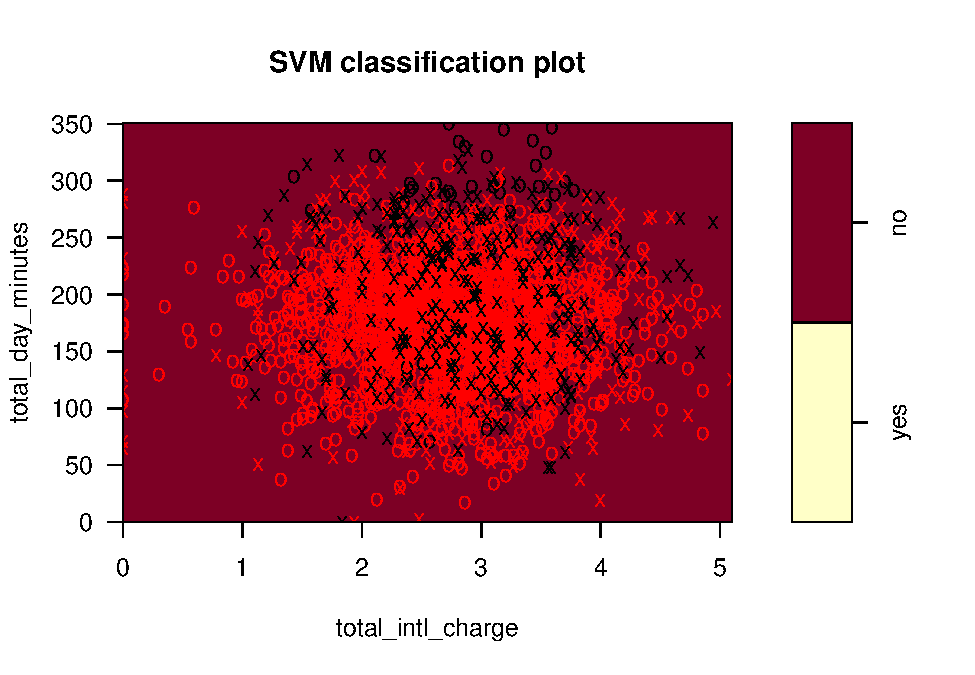
\includegraphics{R_FinalReport_files/figure-latex/unnamed-chunk-5-1.pdf}
红色的支持向量和黑色的数据样例在图中心区域排列很紧密,不能直接分开。

\hypertarget{ux57faux4e8eux652fux6301ux5411ux91cfux673aux8badux7ec3ux6a21ux578bux5b9eux73b0ux7c7bux9884ux6d4b}{%
\subsection{基于支持向量机训练模型实现类预测}\label{ux57faux4e8eux652fux6301ux5411ux91cfux673aux8badux7ec3ux6a21ux578bux5b9eux73b0ux7c7bux9884ux6d4b}}

\begin{enumerate}
\def\labelenumi{\arabic{enumi}.}
\tightlist
\item
  利用已构建的模型和测试数据集预测它的类别
\end{enumerate}

\begin{Shaded}
\begin{Highlighting}[]
\NormalTok{svm.pred=}\KeywordTok{predict}\NormalTok{(model,}
\NormalTok{                 testset[,}\OperatorTok{!}\KeywordTok{names}\NormalTok{(testset) }\OperatorTok\StringTok{ }\KeywordTok{c}\NormalTok{(}\StringTok{"churn"}\NormalTok{)])}
\end{Highlighting}
\end{Shaded}

\begin{enumerate}
\def\labelenumi{\arabic{enumi}.}
\setcounter{enumi}{1}
\tightlist
\item
  建立分类表
\end{enumerate}

\begin{Shaded}
\begin{Highlighting}[]
\NormalTok{svm.table=}\KeywordTok{table}\NormalTok{(svm.pred,}
\NormalTok{                testset}\OperatorTok{$}\NormalTok{churn)}
\end{Highlighting}
\end{Shaded}

\begin{enumerate}
\def\labelenumi{\arabic{enumi}.}
\setcounter{enumi}{2}
\tightlist
\item
  分析一致性系数
\end{enumerate}

\begin{Shaded}
\begin{Highlighting}[]
\KeywordTok{classAgreement}\NormalTok{(svm.table)}
\end{Highlighting}
\end{Shaded}

\begin{verbatim}
## $diag
## [1] 0.9184676
## 
## $kappa
## [1] 0.5855903
## 
## $rand
## [1] 0.850083
## 
## $crand
## [1] 0.5260472
\end{verbatim}

\begin{enumerate}
\def\labelenumi{\arabic{enumi}.}
\setcounter{enumi}{3}
\tightlist
\item
  基于分类表评测预测性能
\end{enumerate}

\begin{Shaded}
\begin{Highlighting}[]
\KeywordTok{library}\NormalTok{(caret)}
\end{Highlighting}
\end{Shaded}

\begin{verbatim}
## Loading required package: lattice
\end{verbatim}

\begin{verbatim}
## Loading required package: ggplot2
\end{verbatim}

\begin{Shaded}
\begin{Highlighting}[]
\KeywordTok{confusionMatrix}\NormalTok{(svm.table)}
\end{Highlighting}
\end{Shaded}

\begin{verbatim}
## Confusion Matrix and Statistics
## 
##         
## svm.pred yes  no
##      yes  70  12
##      no   71 865
##                                           
##                Accuracy : 0.9185          
##                  95% CI : (0.8999, 0.9345)
##     No Information Rate : 0.8615          
##     P-Value [Acc > NIR] : 1.251e-08       
##                                           
##                   Kappa : 0.5856          
##                                           
##  Mcnemar's Test P-Value : 1.936e-10       
##                                           
##             Sensitivity : 0.49645         
##             Specificity : 0.98632         
##          Pos Pred Value : 0.85366         
##          Neg Pred Value : 0.92415         
##              Prevalence : 0.13851         
##          Detection Rate : 0.06876         
##    Detection Prevalence : 0.08055         
##       Balanced Accuracy : 0.74139         
##                                           
##        'Positive' Class : yes             
## 
\end{verbatim}

\hypertarget{ux8c03ux6574ux652fux6301ux5411ux91cfux673a}{%
\subsection{调整支持向量机}\label{ux8c03ux6574ux652fux6301ux5411ux91cfux673a}}

\begin{enumerate}
\def\labelenumi{\arabic{enumi}.}
\tightlist
\item
  tune.svm
\end{enumerate}

\begin{Shaded}
\begin{Highlighting}[]
\NormalTok{tuned=}\KeywordTok{tune.svm}\NormalTok{(churn}\OperatorTok{~}\NormalTok{.,}
               \DataTypeTok{data=}\NormalTok{trainset,}
               \DataTypeTok{gamma=}\DecValTok{10}\OperatorTok{^}\NormalTok{(}\OperatorTok{-}\DecValTok{6}\OperatorTok{:-}\DecValTok{1}\NormalTok{),}
               \DataTypeTok{cost=}\DecValTok{10}\OperatorTok{^}\NormalTok{(}\DecValTok{1}\OperatorTok{:}\DecValTok{2}\NormalTok{))}
\KeywordTok{summary}\NormalTok{(tuned)}
\end{Highlighting}
\end{Shaded}

\begin{verbatim}
## 
## Parameter tuning of 'svm':
## 
## - sampling method: 10-fold cross validation 
## 
## - best parameters:
##  gamma cost
##   0.01  100
## 
## - best performance: 0.07992051 
## 
## - Detailed performance results:
##    gamma cost      error dispersion
## 1  1e-06   10 0.14773474 0.01763545
## 2  1e-05   10 0.14773474 0.01763545
## 3  1e-04   10 0.14773474 0.01763545
## 4  1e-03   10 0.14773474 0.01763545
## 5  1e-02   10 0.09116099 0.02007738
## 6  1e-01   10 0.09288513 0.02507137
## 7  1e-06  100 0.14773474 0.01763545
## 8  1e-05  100 0.14773474 0.01763545
## 9  1e-04  100 0.14773474 0.01763545
## 10 1e-03  100 0.11880505 0.01581561
## 11 1e-02  100 0.07992051 0.02049819
## 12 1e-01  100 0.12226638 0.02627152
\end{verbatim}

\begin{enumerate}
\def\labelenumi{\arabic{enumi}.}
\setcounter{enumi}{2}
\tightlist
\item
  最佳参数设置SVM
\end{enumerate}

\begin{Shaded}
\begin{Highlighting}[]
\NormalTok{model.tuned=}\KeywordTok{svm}\NormalTok{(churn}\OperatorTok{~}\NormalTok{.,}
                \DataTypeTok{data=}\NormalTok{trainset,}
                \DataTypeTok{gamma=}\NormalTok{tuned}\OperatorTok{$}\NormalTok{best.parameters}\OperatorTok{$}\NormalTok{gamma,}
                \DataTypeTok{cost=}\NormalTok{tuned}\OperatorTok{$}\NormalTok{best.parameters}\OperatorTok{$}\NormalTok{cost)}
\KeywordTok{summary}\NormalTok{(model.tuned)}
\end{Highlighting}
\end{Shaded}

\begin{verbatim}
## 
## Call:
## svm(formula = churn ~ ., data = trainset, gamma = tuned$best.parameters$gamma, 
##     cost = tuned$best.parameters$cost)
## 
## 
## Parameters:
##    SVM-Type:  C-classification 
##  SVM-Kernel:  radial 
##        cost:  100 
## 
## Number of Support Vectors:  547
## 
##  ( 304 243 )
## 
## 
## Number of Classes:  2 
## 
## Levels: 
##  yes no
\end{verbatim}

\begin{enumerate}
\def\labelenumi{\arabic{enumi}.}
\setcounter{enumi}{3}
\tightlist
\item
  类标号预测
\end{enumerate}

\begin{Shaded}
\begin{Highlighting}[]
\NormalTok{svm.tuned.pred=}\KeywordTok{predict}\NormalTok{(model.tuned,}
\NormalTok{                       testset[, }\OperatorTok{!}\KeywordTok{names}\NormalTok{(testset) }\OperatorTok\StringTok{ }\KeywordTok{c}\NormalTok{(}\StringTok{"churn"}\NormalTok{)])}
\end{Highlighting}
\end{Shaded}

\begin{enumerate}
\def\labelenumi{\arabic{enumi}.}
\setcounter{enumi}{4}
\tightlist
\item
  分类表
\end{enumerate}

\begin{Shaded}
\begin{Highlighting}[]
\NormalTok{svm.tuned.table=}\KeywordTok{table}\NormalTok{(svm.tuned.pred,}
\NormalTok{                      testset}\OperatorTok{$}\NormalTok{churn)}
\NormalTok{svm.tuned.table}
\end{Highlighting}
\end{Shaded}

\begin{verbatim}
##               
## svm.tuned.pred yes  no
##            yes  95  24
##            no   46 853
\end{verbatim}

\begin{enumerate}
\def\labelenumi{\arabic{enumi}.}
\setcounter{enumi}{5}
\tightlist
\item
  得到相关系数,完成算法性能评测
\end{enumerate}

\begin{Shaded}
\begin{Highlighting}[]
\KeywordTok{classAgreement}\NormalTok{(svm.tuned.table)}
\end{Highlighting}
\end{Shaded}

\begin{verbatim}
## $diag
## [1] 0.9312377
## 
## $kappa
## [1] 0.691678
## 
## $rand
## [1] 0.871806
## 
## $crand
## [1] 0.6303615
\end{verbatim}

\begin{enumerate}
\def\labelenumi{\arabic{enumi}.}
\setcounter{enumi}{6}
\tightlist
\item
  评测优化后的模型性能
\end{enumerate}

\begin{Shaded}
\begin{Highlighting}[]
\KeywordTok{confusionMatrix}\NormalTok{(svm.tuned.table)}
\end{Highlighting}
\end{Shaded}

\begin{verbatim}
## Confusion Matrix and Statistics
## 
##               
## svm.tuned.pred yes  no
##            yes  95  24
##            no   46 853
##                                          
##                Accuracy : 0.9312         
##                  95% CI : (0.9139, 0.946)
##     No Information Rate : 0.8615         
##     P-Value [Acc > NIR] : 1.56e-12       
##                                          
##                   Kappa : 0.6917         
##                                          
##  Mcnemar's Test P-Value : 0.01207        
##                                          
##             Sensitivity : 0.67376        
##             Specificity : 0.97263        
##          Pos Pred Value : 0.79832        
##          Neg Pred Value : 0.94883        
##              Prevalence : 0.13851        
##          Detection Rate : 0.09332        
##    Detection Prevalence : 0.11690        
##       Balanced Accuracy : 0.82320        
##                                          
##        'Positive' Class : yes            
## 
\end{verbatim}

试错法寻找最佳的gamma和惩罚因子。

\hypertarget{ux6a21ux578bux7684ux7ed3ux679cux5206ux6790ux4e0eux89e3ux91ca}{%
\section{模型的结果分析与解释}\label{ux6a21ux578bux7684ux7ed3ux679cux5206ux6790ux4e0eux89e3ux91ca}}

\hypertarget{ux6a21ux578bux8bc4ux4f30}{%
\subsection{模型评估}\label{ux6a21ux578bux8bc4ux4f30}}

\hypertarget{ux57faux4e8ekux6298ux4ea4ux53c9ux9a8cux8bc1ux65b9ux6cd5ux8bc4ux6d4bux6a21ux578bux6027ux80fd}{%
\subsubsection{基于k折交叉验证方法评测模型性能}\label{ux57faux4e8ekux6298ux4ea4ux53c9ux9a8cux8bc1ux65b9ux6cd5ux8bc4ux6d4bux6a21ux578bux6027ux80fd}}

\begin{Shaded}
\begin{Highlighting}[]
\CommentTok{#索引分成10份}
\NormalTok{ind=}\KeywordTok{cut}\NormalTok{(}\DecValTok{1}\OperatorTok{:}\KeywordTok{nrow}\NormalTok{(churnTrain),}
        \DataTypeTok{breaks=}\DecValTok{10}\NormalTok{,}
        \DataTypeTok{labels=}\NormalTok{F)}

\CommentTok{#SVM依赖}
\KeywordTok{library}\NormalTok{(e1071)}
\CommentTok{#10折交叉验证}
\NormalTok{accuracies=}\KeywordTok{c}\NormalTok{()}
\ControlFlowTok{for}\NormalTok{ (i }\ControlFlowTok{in} \DecValTok{1}\OperatorTok{:}\DecValTok{10}\NormalTok{)\{}
\NormalTok{  fit=}\KeywordTok{svm}\NormalTok{(churn}\OperatorTok{~}\NormalTok{.,}
\NormalTok{          churnTrain[ind}\OperatorTok{!=}\NormalTok{i,])}
\NormalTok{  predictions=}\KeywordTok{predict}\NormalTok{(fit,}
\NormalTok{                      churnTrain[ind}\OperatorTok{==}\NormalTok{i, }\OperatorTok{!}\KeywordTok{names}\NormalTok{(churnTrain) }\OperatorTok\StringTok{ }\KeywordTok{c}\NormalTok{(}\StringTok{"churn"}\NormalTok{)])}
\NormalTok{  correct_count=}\KeywordTok{sum}\NormalTok{(predictions}\OperatorTok{==}\NormalTok{churnTrain[ind}\OperatorTok{==}\StringTok{ }\NormalTok{i,}\KeywordTok{c}\NormalTok{(}\StringTok{"churn"}\NormalTok{)])}
\NormalTok{  accuracies=}\StringTok{ }\KeywordTok{append}\NormalTok{(correct_count}\OperatorTok{/}\KeywordTok{nrow}\NormalTok{(churnTrain[ind}\OperatorTok{==}\NormalTok{i,]),}
\NormalTok{                     accuracies)}
\NormalTok{\}}

\CommentTok{#输出准确率}
\NormalTok{accuracies}
\end{Highlighting}
\end{Shaded}

\begin{verbatim}
##  [1] 0.9341317 0.8948949 0.8978979 0.9459459 0.9219219 0.9281437 0.9219219
##  [8] 0.9249249 0.9189189 0.9251497
\end{verbatim}

\begin{Shaded}
\begin{Highlighting}[]
\KeywordTok{mean}\NormalTok{(accuracies)}
\end{Highlighting}
\end{Shaded}

\begin{verbatim}
## [1] 0.9213852
\end{verbatim}

\hypertarget{ux5229ux7528e1071ux5305ux5b8cux6210ux4ea4ux53c9ux9a8cux8bc1}{%
\subsubsection{利用e1071包完成交叉验证}\label{ux5229ux7528e1071ux5305ux5b8cux6210ux4ea4ux53c9ux9a8cux8bc1}}

tuning函数获取最小误差值。

\begin{Shaded}
\begin{Highlighting}[]
\NormalTok{tuned=}\KeywordTok{tune.svm}\NormalTok{(churn}\OperatorTok{~}\NormalTok{.,}
               \DataTypeTok{data=}\NormalTok{trainset,}
               \DataTypeTok{gamma=}\DecValTok{10}\OperatorTok{^-}\DecValTok{2}\NormalTok{,}
               \DataTypeTok{cost=}\DecValTok{10}\OperatorTok{^-}\DecValTok{2}\NormalTok{,}
               \DataTypeTok{tunecontrol=}\KeywordTok{tune.control}\NormalTok{(}\DataTypeTok{cross=}\DecValTok{10}\NormalTok{))}

\KeywordTok{summary}\NormalTok{(tuned)}
\end{Highlighting}
\end{Shaded}

\begin{verbatim}
## 
## Error estimation of 'svm' using 10-fold cross validation: 0.1477142
\end{verbatim}

\begin{enumerate}
\def\labelenumi{\arabic{enumi}.}
\setcounter{enumi}{2}
\tightlist
\item
  模型的性能细节
\end{enumerate}

\begin{Shaded}
\begin{Highlighting}[]
\NormalTok{tuned}\OperatorTok{$}\NormalTok{performances}
\end{Highlighting}
\end{Shaded}

\begin{verbatim}
##   gamma cost     error dispersion
## 1  0.01 0.01 0.1477142  0.0258799
\end{verbatim}

\begin{enumerate}
\def\labelenumi{\arabic{enumi}.}
\setcounter{enumi}{3}
\tightlist
\item
  使用优化后的模型产生分类表
\end{enumerate}

\begin{Shaded}
\begin{Highlighting}[]
\NormalTok{svmfit=tuned}\OperatorTok{$}\NormalTok{best.model}
\KeywordTok{table}\NormalTok{(trainset[,}\KeywordTok{c}\NormalTok{(}\StringTok{"churn"}\NormalTok{)],}
      \KeywordTok{predict}\NormalTok{(svmfit))}
\end{Highlighting}
\end{Shaded}

\begin{verbatim}
##      
##        yes   no
##   yes    0  342
##   no     0 1973
\end{verbatim}

\hypertarget{ux5229ux7528caretux5305ux5b8cux6210ux4ea4ux53c9ux68c0ux9a8c}{%
\subsubsection{利用caret包完成交叉检验}\label{ux5229ux7528caretux5305ux5b8cux6210ux4ea4ux53c9ux68c0ux9a8c}}

\begin{Shaded}
\begin{Highlighting}[]
\CommentTok{#install.packages("caret")}
\KeywordTok{library}\NormalTok{(caret)}

\CommentTok{#重复的k折交叉验证,被用于检测模型的稳定性。如果稳定,用户将得到类似的测试结果。}
\CommentTok{#设置控制训练参数,进行重复3次的10折交叉验证}
\NormalTok{control=}\KeywordTok{trainControl}\NormalTok{(}\DataTypeTok{method=}\StringTok{"repeatedcv"}\NormalTok{,}
                     \DataTypeTok{number=}\DecValTok{10}\NormalTok{,}
                     \DataTypeTok{repeats=}\DecValTok{3}\NormalTok{)}


\NormalTok{model=}\KeywordTok{train}\NormalTok{(churn}\OperatorTok{~}\NormalTok{.,}
            \DataTypeTok{data=}\NormalTok{trainset,}
            \DataTypeTok{method=}\StringTok{"rpart"}\NormalTok{,}
            \DataTypeTok{preProcess=}\StringTok{"scale"}\NormalTok{,}
            \DataTypeTok{trControl=}\NormalTok{control)}

\NormalTok{model}
\end{Highlighting}
\end{Shaded}

\begin{verbatim}
## CART 
## 
## 2315 samples
##   16 predictor
##    2 classes: 'yes', 'no' 
## 
## Pre-processing: scaled (16) 
## Resampling: Cross-Validated (10 fold, repeated 3 times) 
## Summary of sample sizes: 2083, 2083, 2084, 2084, 2084, 2084, ... 
## Resampling results across tuning parameters:
## 
##   cp          Accuracy   Kappa    
##   0.05555556  0.9072814  0.5580218
##   0.07456140  0.8711367  0.3141883
##   0.07602339  0.8621988  0.2009855
## 
## Accuracy was used to select the optimal model using the largest value.
## The final value used for the model was cp = 0.05555556.
\end{verbatim}

模型输出了3次重新采样的结果,其中cp为0.555的模型准确率最高。 \#\#\#
利用caret包对变量重要程度排序
比较给定模型输出效果的变化敏感程度来评估不同特征对模型的重要性。

\begin{Shaded}
\begin{Highlighting}[]
\NormalTok{importance=}\KeywordTok{varImp}\NormalTok{(model,}\DataTypeTok{scale=}\OtherTok{FALSE}\NormalTok{)}
\NormalTok{importance}
\end{Highlighting}
\end{Shaded}

\begin{verbatim}
## rpart variable importance
## 
##                               Overall
## number_customer_service_calls 116.015
## total_day_minutes             106.988
## total_day_charge              100.648
## international_planyes          86.789
## voice_mail_planyes             25.974
## total_eve_charge               23.097
## total_eve_minutes              23.097
## number_vmail_messages          19.885
## total_intl_minutes              6.347
## total_day_calls                 0.000
## total_night_minutes             0.000
## total_eve_calls                 0.000
## total_intl_charge               0.000
## total_night_charge              0.000
## total_night_calls               0.000
## total_intl_calls                0.000
\end{verbatim}

\begin{Shaded}
\begin{Highlighting}[]
\KeywordTok{plot}\NormalTok{(importance)}
\end{Highlighting}
\end{Shaded}

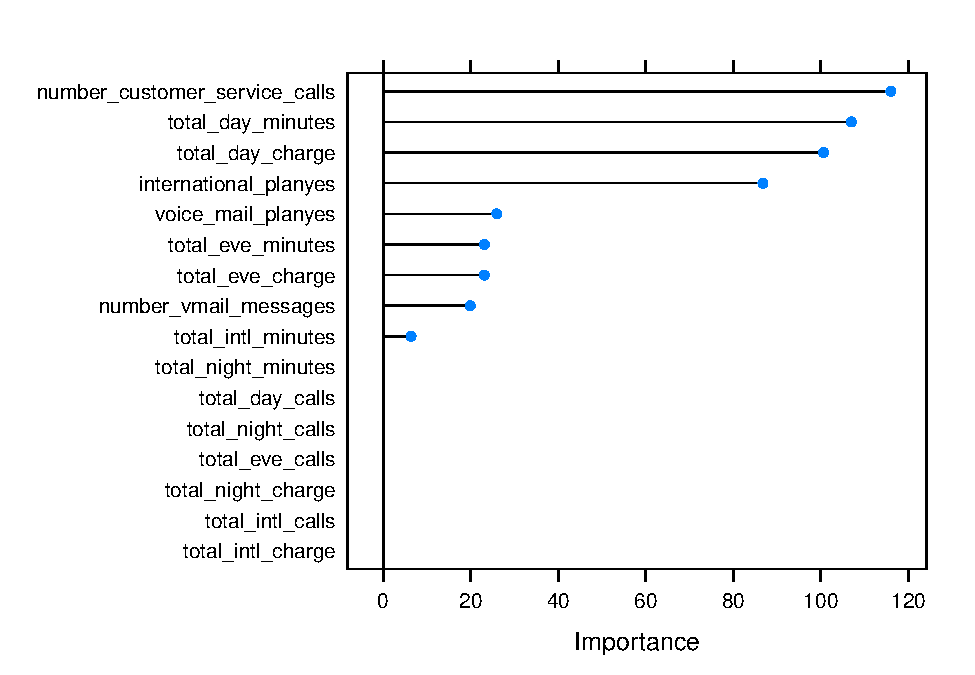
\includegraphics{R_FinalReport_files/figure-latex/unnamed-chunk-22-1.pdf}

\hypertarget{ux5229ux7528caretux5305ux627eux5230ux9ad8ux5ea6ux5173ux8054ux7684ux7279ux5f81}{%
\subsubsection{利用caret包找到高度关联的特征}\label{ux5229ux7528caretux5305ux627eux5230ux9ad8ux5ea6ux5173ux8054ux7684ux7279ux5f81}}

如果能提前去掉高度关联的属性,训练模型的性能会更好。

\begin{Shaded}
\begin{Highlighting}[]
\CommentTok{#去掉非数值类型的属性}
\NormalTok{new_train=trainset[, }\OperatorTok{!}\KeywordTok{names}\NormalTok{(churnTrain)  }\OperatorTok\StringTok{ }\KeywordTok{c}\NormalTok{(}\StringTok{"churn"}\NormalTok{,}\StringTok{"international_plan"}\NormalTok{,}\StringTok{"voice_mail_plan"}\NormalTok{)]}

\CommentTok{#计算每个属性之间的关联度}
\NormalTok{cor_mat=}\KeywordTok{cor}\NormalTok{(new_train)}

\CommentTok{#找到关联度超过0.75的属性}
\NormalTok{highlyCorrelated=}\KeywordTok{findCorrelation}\NormalTok{(cor_mat,}\DataTypeTok{cutoff=}\FloatTok{0.75}\NormalTok{)}

\KeywordTok{names}\NormalTok{(new_train)[highlyCorrelated]}
\end{Highlighting}
\end{Shaded}

\begin{verbatim}
## [1] "total_intl_minutes"  "total_day_charge"    "total_eve_minutes"  
## [4] "total_night_minutes"
\end{verbatim}

\hypertarget{ux5229ux7528caretux5305ux9009ux62e9ux7279ux5f81}{%
\subsubsection{利用caret包选择特征}\label{ux5229ux7528caretux5305ux9009ux62e9ux7279ux5f81}}

递归特征排除函数\texttt{rfe}

\begin{Shaded}
\begin{Highlighting}[]
\CommentTok{#international_plan的特征转换为intl_yes和Intl_no}
\NormalTok{intl_plan=}\KeywordTok{model.matrix}\NormalTok{(}\OperatorTok{~}\StringTok{ }\NormalTok{trainset.international_plan }\OperatorTok{-}\StringTok{ }\DecValTok{1}\NormalTok{,}
                       \DataTypeTok{data=}\KeywordTok{data.frame}\NormalTok{(trainset}\OperatorTok{$}\NormalTok{international_plan))}

\KeywordTok{colnames}\NormalTok{(intl_plan)=}\KeywordTok{c}\NormalTok{(}\StringTok{"trainset.international_planno"}\NormalTok{=}\StringTok{"intl_no"}\NormalTok{,}
                      \StringTok{"trainset.international_planyes"}\NormalTok{=}\StringTok{"intl_yes"}\NormalTok{)}


\CommentTok{#voice_mail_plan的特征转换为voice_yes和voice_no}
\NormalTok{voice_plan=}\KeywordTok{model.matrix}\NormalTok{(}\OperatorTok{~}\StringTok{ }\NormalTok{trainset.voice_mail_plan}\DecValTok{-1}\NormalTok{,}
                        \DataTypeTok{data=}\KeywordTok{data.frame}\NormalTok{(trainset}\OperatorTok{$}\NormalTok{voice_mail_plan))}

\KeywordTok{colnames}\NormalTok{(voice_plan)=}\KeywordTok{c}\NormalTok{(}\StringTok{"trainset.voice_planno"}\NormalTok{=}\StringTok{"voice_no"}\NormalTok{,}
                       \StringTok{"trainset.voice_planyes"}\NormalTok{=}\StringTok{"voice_yes"}\NormalTok{)}

\CommentTok{#去掉2个属性,并将训练数据与两个数据框合并}
\NormalTok{trainset}\OperatorTok{$}\NormalTok{international_plan=}\OtherTok{NULL}
\NormalTok{trainset}\OperatorTok{$}\NormalTok{voice_mail_plan=}\OtherTok{NULL}
\NormalTok{trainset=}\KeywordTok{cbind}\NormalTok{(intl_plan,voice_plan,trainset)}

\CommentTok{#test数据集同理如上}
\NormalTok{intl_plan=}\KeywordTok{model.matrix}\NormalTok{(}\OperatorTok{~}\StringTok{ }\NormalTok{testset.international_plan }\OperatorTok{-}\StringTok{ }\DecValTok{1}\NormalTok{,}
                       \DataTypeTok{data=}\KeywordTok{data.frame}\NormalTok{(testset}\OperatorTok{$}\NormalTok{international_plan))}

\KeywordTok{colnames}\NormalTok{(intl_plan)=}\KeywordTok{c}\NormalTok{(}\StringTok{"testset.international_planno"}\NormalTok{=}\StringTok{"intl_no"}\NormalTok{,}
                      \StringTok{"testset.international_planyes"}\NormalTok{=}\StringTok{"intl_yes"}\NormalTok{)}


\NormalTok{voice_plan=}\KeywordTok{model.matrix}\NormalTok{(}\OperatorTok{~}\StringTok{ }\NormalTok{testset.voice_mail_plan}\DecValTok{-1}\NormalTok{, }\DataTypeTok{data=}\KeywordTok{data.frame}\NormalTok{(testset}\OperatorTok{$}\NormalTok{voice_mail_plan))}

\KeywordTok{colnames}\NormalTok{(voice_plan)=}\KeywordTok{c}\NormalTok{(}\StringTok{"testset.voice_planno"}\NormalTok{=}\StringTok{"voice_no"}\NormalTok{,}
                       \StringTok{"testset.voice_planyes"}\NormalTok{=}\StringTok{"voice_yes"}\NormalTok{)}


\NormalTok{testset}\OperatorTok{$}\NormalTok{international_plan=}\OtherTok{NULL}
\NormalTok{testset}\OperatorTok{$}\NormalTok{voice_mail_plan=}\OtherTok{NULL}
\NormalTok{testset=}\KeywordTok{cbind}\NormalTok{(intl_plan,voice_plan,testset)}
\end{Highlighting}
\end{Shaded}

\begin{enumerate}
\def\labelenumi{\arabic{enumi}.}
\setcounter{enumi}{6}
\tightlist
\item
  使用LDA创建一个特征筛选
\end{enumerate}

\begin{Shaded}
\begin{Highlighting}[]
\NormalTok{ldaControl=}\KeywordTok{rfeControl}\NormalTok{(}\DataTypeTok{functions =}\NormalTok{ ldaFuncs,}\DataTypeTok{method=}\StringTok{"cv"}\NormalTok{)}
\end{Highlighting}
\end{Shaded}

\begin{enumerate}
\def\labelenumi{\arabic{enumi}.}
\setcounter{enumi}{7}
\tightlist
\item
  利用从编号1-18的数据子集对训练数据集trainset进行反向特征筛选
\end{enumerate}

\begin{Shaded}
\begin{Highlighting}[]
\NormalTok{ldaProfile=}\KeywordTok{rfe}\NormalTok{(trainset[, }\OperatorTok{!}\KeywordTok{names}\NormalTok{(trainset) }\OperatorTok\StringTok{ }\KeywordTok{c}\NormalTok{(}\StringTok{"churn"}\NormalTok{)],trainset[,}\KeywordTok{c}\NormalTok{(}\StringTok{"churn"}\NormalTok{)],}
               \DataTypeTok{sizes =} \KeywordTok{c}\NormalTok{(}\DecValTok{1}\OperatorTok{:}\DecValTok{18}\NormalTok{),}
               \DataTypeTok{rfeControl =}\NormalTok{ ldaControl)}

\NormalTok{ldaProfile}
\end{Highlighting}
\end{Shaded}

\begin{verbatim}
## 
## Recursive feature selection
## 
## Outer resampling method: Cross-Validated (10 fold) 
## 
## Resampling performance over subset size:
## 
##  Variables Accuracy    Kappa AccuracySD KappaSD Selected
##          1   0.8531 0.009672   0.001767 0.02039         
##          2   0.8531 0.009829   0.002581 0.02072         
##          3   0.8367 0.130371   0.017907 0.09934         
##          4   0.8406 0.204617   0.021050 0.10803         
##          5   0.8467 0.226621   0.024150 0.14245         
##          6   0.8449 0.219809   0.021163 0.11980         
##          7   0.8441 0.216697   0.021582 0.12753         
##          8   0.8437 0.216058   0.025947 0.14637         
##          9   0.8471 0.236037   0.027635 0.14082         
##         10   0.8480 0.237765   0.026364 0.14168         
##         11   0.8475 0.235295   0.027232 0.14220         
##         12   0.8488 0.242297   0.027482 0.14613         
##         13   0.8501 0.251306   0.027321 0.14812         
##         14   0.8523 0.255369   0.026387 0.15208         
##         15   0.8540 0.266462   0.026225 0.15073        *
##         16   0.8527 0.258823   0.024326 0.14263         
##         17   0.8506 0.252423   0.025551 0.14221         
##         18   0.8514 0.254383   0.025252 0.14281         
## 
## The top 5 variables (out of 15):
##    total_day_charge, total_day_minutes, intl_yes, intl_no, number_customer_service_calls
\end{verbatim}

\begin{enumerate}
\def\labelenumi{\arabic{enumi}.}
\setcounter{enumi}{8}
\tightlist
\item
  选择结果
\end{enumerate}

\begin{Shaded}
\begin{Highlighting}[]
\KeywordTok{plot}\NormalTok{(ldaProfile,}\DataTypeTok{type=}\KeywordTok{c}\NormalTok{(}\StringTok{"o"}\NormalTok{,}\StringTok{"g"}\NormalTok{))}
\end{Highlighting}
\end{Shaded}

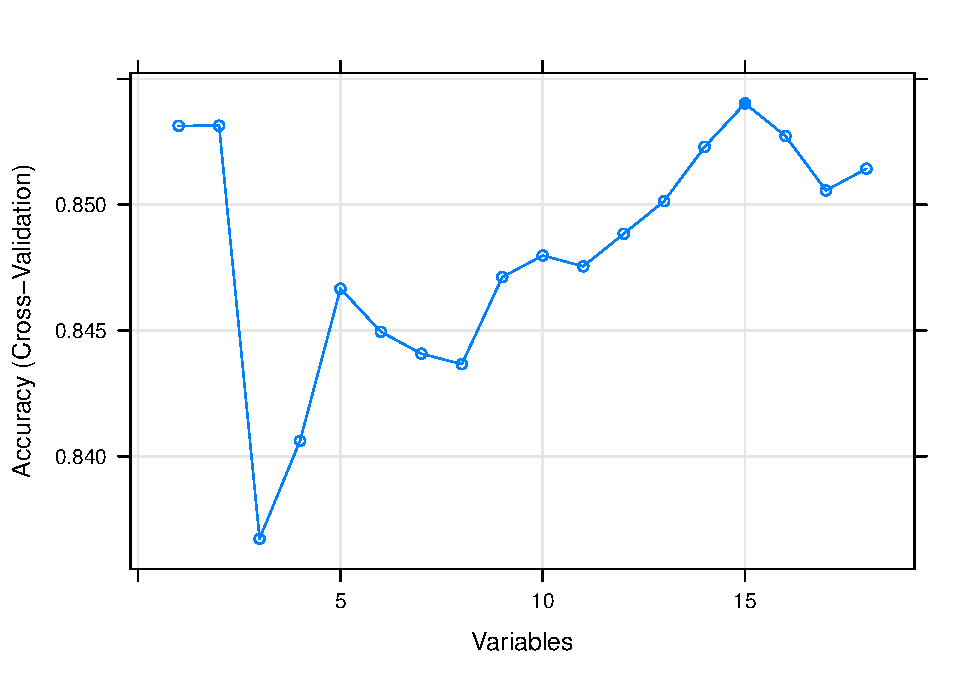
\includegraphics{R_FinalReport_files/figure-latex/unnamed-chunk-27-1.pdf}

\begin{enumerate}
\def\labelenumi{\arabic{enumi}.}
\setcounter{enumi}{9}
\tightlist
\item
  检测最佳变量子集
\end{enumerate}

\begin{Shaded}
\begin{Highlighting}[]
\NormalTok{ldaProfile}\OperatorTok{$}\NormalTok{optVariables}
\end{Highlighting}
\end{Shaded}

\begin{verbatim}
##  [1] "total_day_charge"              "total_day_minutes"            
##  [3] "intl_yes"                      "intl_no"                      
##  [5] "number_customer_service_calls" "total_eve_minutes"            
##  [7] "total_eve_charge"              "total_intl_calls"             
##  [9] "voice_yes"                     "voice_no"                     
## [11] "number_vmail_messages"         "total_intl_charge"            
## [13] "total_intl_minutes"            "total_night_charge"           
## [15] "total_night_minutes"
\end{verbatim}

\begin{enumerate}
\def\labelenumi{\arabic{enumi}.}
\setcounter{enumi}{10}
\tightlist
\item
  检测合适的模型
\end{enumerate}

\begin{Shaded}
\begin{Highlighting}[]
\NormalTok{ldaProfile}\OperatorTok{$}\NormalTok{fit}
\end{Highlighting}
\end{Shaded}

\begin{verbatim}
## Call:
## lda(x, y)
## 
## Prior probabilities of groups:
##       yes        no 
## 0.1477322 0.8522678 
## 
## Group means:
##     total_day_charge total_day_minutes   intl_yes   intl_no
## yes         35.00143          205.8877 0.29532164 0.7046784
## no          29.62402          174.2555 0.06487582 0.9351242
##     number_customer_service_calls total_eve_minutes total_eve_charge
## yes                      2.204678          213.7269         18.16702
## no                       1.441460          199.6197         16.96789
##     total_intl_calls voice_yes  voice_no number_vmail_messages
## yes         4.134503 0.1666667 0.8333333              5.099415
## no          4.514445 0.2954891 0.7045109              8.674607
##     total_intl_charge total_intl_minutes total_night_charge total_night_minutes
## yes          2.899386           10.73684           9.245994            205.4640
## no           2.741343           10.15119           9.063882            201.4184
## 
## Coefficients of linear discriminants:
##                                         LD1
## total_day_charge                0.671376021
## total_day_minutes              -0.123085519
## intl_yes                       -1.130269257
## intl_no                         1.130269257
## number_customer_service_calls  -0.421346323
## total_eve_minutes               0.183124313
## total_eve_charge               -2.210668112
## total_intl_calls                0.066574547
## voice_yes                       0.330197066
## voice_no                       -0.330197066
## number_vmail_messages          -0.003558459
## total_intl_charge               2.316437631
## total_intl_minutes             -0.694000839
## total_night_charge            -14.513932481
## total_night_minutes             0.651028494
\end{verbatim}

\begin{enumerate}
\def\labelenumi{\arabic{enumi}.}
\setcounter{enumi}{11}
\tightlist
\item
  重采样评估模型
\end{enumerate}

\begin{Shaded}
\begin{Highlighting}[]
\KeywordTok{postResample}\NormalTok{(}\KeywordTok{predict}\NormalTok{(ldaProfile,}
\NormalTok{                     testset[, }\OperatorTok{!}\KeywordTok{names}\NormalTok{(testset) }\OperatorTok\StringTok{ }\KeywordTok{c}\NormalTok{(}\StringTok{"churn"}\NormalTok{)]),}
\NormalTok{             testset[,}\KeywordTok{c}\NormalTok{(}\StringTok{"churn"}\NormalTok{)])}
\end{Highlighting}
\end{Shaded}

\begin{verbatim}
##  Accuracy     Kappa 
## 0.8585462 0.2568816
\end{verbatim}

\hypertarget{ux8bc4ux6d4bux56deux5f52ux6a21ux578bux7684ux6027ux80fd}{%
\subsubsection{评测回归模型的性能}\label{ux8bc4ux6d4bux56deux5f52ux6a21ux578bux7684ux6027ux80fd}}

相对平方差(Relative Square Error)。 数据换用Quartet数据集。

\begin{Shaded}
\begin{Highlighting}[]
\CommentTok{#install.packages("car")}
\KeywordTok{library}\NormalTok{(car)}
\end{Highlighting}
\end{Shaded}

\begin{verbatim}
## Loading required package: carData
\end{verbatim}

\begin{Shaded}
\begin{Highlighting}[]
\KeywordTok{data}\NormalTok{(Quartet)}

\KeywordTok{plot}\NormalTok{(Quartet}\OperatorTok{$}\NormalTok{x,Quartet}\OperatorTok{$}\NormalTok{y3)}
\NormalTok{lmfit=}\KeywordTok{lm}\NormalTok{(Quartet}\OperatorTok{$}\NormalTok{y3}\OperatorTok{~}\NormalTok{Quartet}\OperatorTok{$}\NormalTok{x)}
\KeywordTok{abline}\NormalTok{(lmfit,}\DataTypeTok{col=}\StringTok{"red"}\NormalTok{)}
\end{Highlighting}
\end{Shaded}

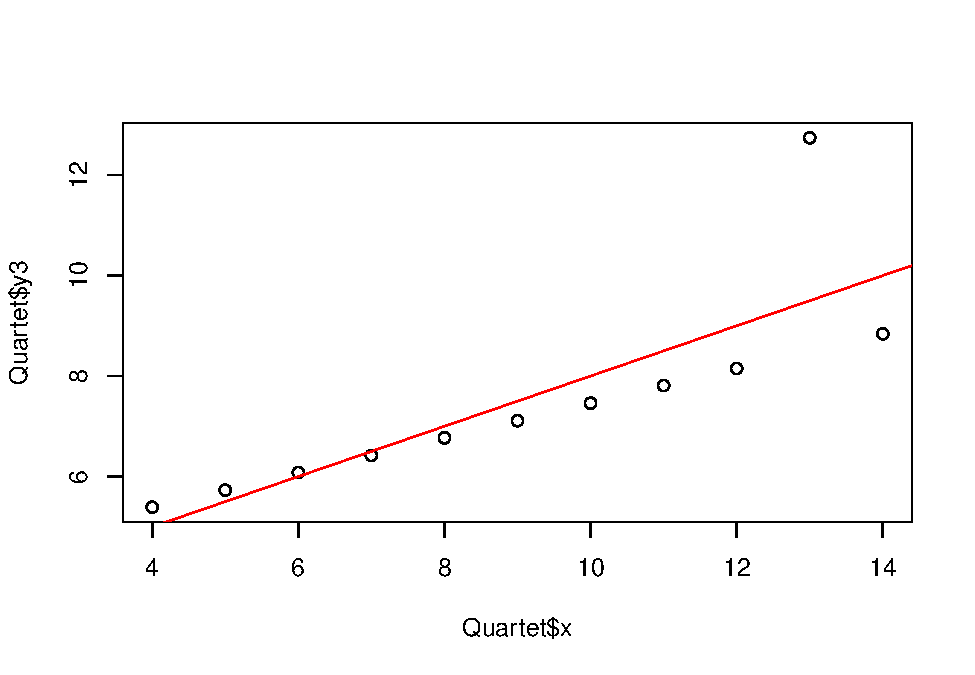
\includegraphics{R_FinalReport_files/figure-latex/unnamed-chunk-31-1.pdf}

\begin{enumerate}
\def\labelenumi{\arabic{enumi}.}
\setcounter{enumi}{2}
\tightlist
\item
  预测结果
\end{enumerate}

\begin{Shaded}
\begin{Highlighting}[]
\NormalTok{predicted=}\KeywordTok{predict}\NormalTok{(lmfit,}\DataTypeTok{newdata=}\NormalTok{Quartet[}\KeywordTok{c}\NormalTok{(}\StringTok{"x"}\NormalTok{)])}
\end{Highlighting}
\end{Shaded}

4.均方误差

\begin{Shaded}
\begin{Highlighting}[]
\NormalTok{actual=Quartet}\OperatorTok{$}\NormalTok{y3}
\NormalTok{rmse=(}\KeywordTok{mean}\NormalTok{((predicted}\OperatorTok{-}\NormalTok{actual)}\OperatorTok{^}\DecValTok{2}\NormalTok{))}\OperatorTok{^}\FloatTok{0.5}
\NormalTok{rmse}
\end{Highlighting}
\end{Shaded}

\begin{verbatim}
## [1] 1.118286
\end{verbatim}

\begin{enumerate}
\def\labelenumi{\arabic{enumi}.}
\setcounter{enumi}{4}
\tightlist
\item
  相对平方误差
\end{enumerate}

\begin{Shaded}
\begin{Highlighting}[]
\NormalTok{mu=}\KeywordTok{mean}\NormalTok{(actual)}
\NormalTok{rse=}\KeywordTok{mean}\NormalTok{((predicted}\OperatorTok{-}\NormalTok{actual)}\OperatorTok{^}\DecValTok{2}\NormalTok{)}\OperatorTok{/}\KeywordTok{mean}\NormalTok{((mu}\OperatorTok{-}\NormalTok{actual)}\OperatorTok{^}\DecValTok{2}\NormalTok{)}
\NormalTok{rse}
\end{Highlighting}
\end{Shaded}

\begin{verbatim}
## [1] 0.333676
\end{verbatim}

\begin{enumerate}
\def\labelenumi{\arabic{enumi}.}
\setcounter{enumi}{5}
\tightlist
\item
  \(R^2\)
\end{enumerate}

\begin{Shaded}
\begin{Highlighting}[]
\NormalTok{rsquare=}\DecValTok{1}\OperatorTok{-}\NormalTok{rse}
\NormalTok{rsquare}
\end{Highlighting}
\end{Shaded}

\begin{verbatim}
## [1] 0.666324
\end{verbatim}

\begin{enumerate}
\def\labelenumi{\arabic{enumi}.}
\setcounter{enumi}{6}
\tightlist
\item
  采用MASS包重新计算y3的值。用模糊线性回归处理数据集。
\end{enumerate}

\begin{Shaded}
\begin{Highlighting}[]
\KeywordTok{library}\NormalTok{(MASS)}
\KeywordTok{plot}\NormalTok{(Quartet}\OperatorTok{$}\NormalTok{x,Quartet}\OperatorTok{$}\NormalTok{y3)}
\NormalTok{rlmfit=}\KeywordTok{rlm}\NormalTok{(Quartet}\OperatorTok{$}\NormalTok{y3}\OperatorTok{~}\NormalTok{Quartet}\OperatorTok{$}\NormalTok{x)}
\KeywordTok{abline}\NormalTok{(rlmfit, }\DataTypeTok{col=}\StringTok{"red"}\NormalTok{)}
\end{Highlighting}
\end{Shaded}

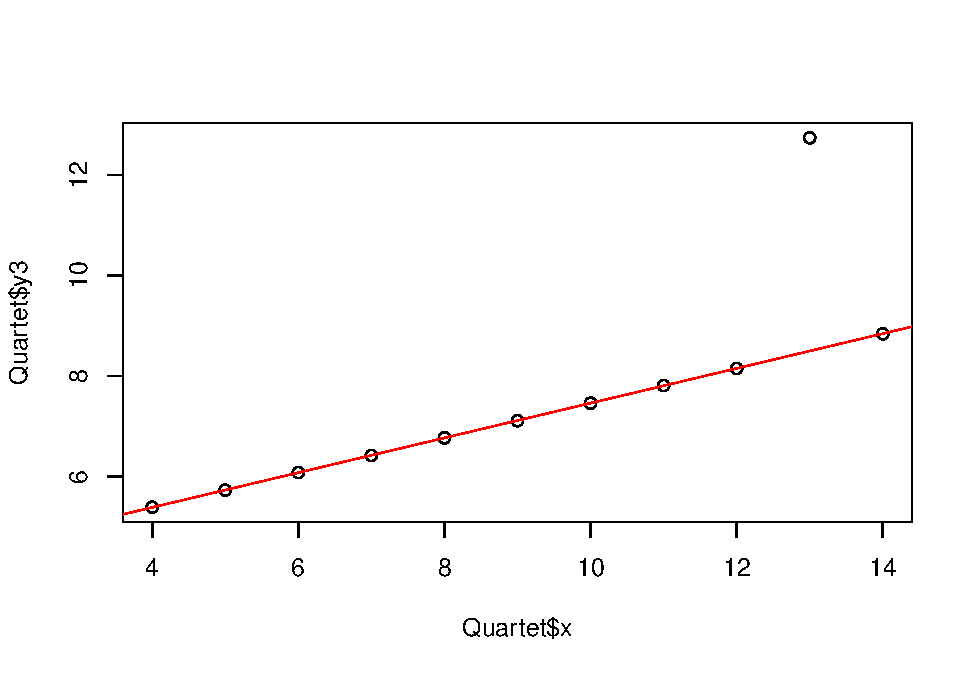
\includegraphics{R_FinalReport_files/figure-latex/unnamed-chunk-36-1.pdf}

\begin{enumerate}
\def\labelenumi{\arabic{enumi}.}
\setcounter{enumi}{7}
\tightlist
\item
  预测
\end{enumerate}

\begin{Shaded}
\begin{Highlighting}[]
\NormalTok{predicted=}\KeywordTok{predict}\NormalTok{(rlmfit,}\DataTypeTok{newdata =}\NormalTok{ Quartet[}\KeywordTok{c}\NormalTok{(}\StringTok{"x"}\NormalTok{)])}
\end{Highlighting}
\end{Shaded}

\begin{enumerate}
\def\labelenumi{\arabic{enumi}.}
\setcounter{enumi}{8}
\tightlist
\item
  均方根误差
\end{enumerate}

\begin{Shaded}
\begin{Highlighting}[]
\NormalTok{actual=Quartet}\OperatorTok{$}\NormalTok{y3}
\NormalTok{rmse=(}\KeywordTok{mean}\NormalTok{((predicted}\OperatorTok{-}\NormalTok{actual)}\OperatorTok{^}\DecValTok{2}\NormalTok{))}\OperatorTok{^}\FloatTok{0.5}
\NormalTok{rmse}
\end{Highlighting}
\end{Shaded}

\begin{verbatim}
## [1] 1.279045
\end{verbatim}

\begin{enumerate}
\def\labelenumi{\arabic{enumi}.}
\setcounter{enumi}{9}
\tightlist
\item
  相对平方误差
\end{enumerate}

\begin{Shaded}
\begin{Highlighting}[]
\NormalTok{mu=}\KeywordTok{mean}\NormalTok{(actual)}
\NormalTok{rse=}\KeywordTok{mean}\NormalTok{((predicted}\OperatorTok{-}\NormalTok{actual)}\OperatorTok{^}\DecValTok{2}\NormalTok{)}\OperatorTok{/}\KeywordTok{mean}\NormalTok{((mu}\OperatorTok{-}\NormalTok{actual)}\OperatorTok{^}\DecValTok{2}\NormalTok{)}
\NormalTok{rse}
\end{Highlighting}
\end{Shaded}

\begin{verbatim}
## [1] 0.4365067
\end{verbatim}

\begin{enumerate}
\def\labelenumi{\arabic{enumi}.}
\setcounter{enumi}{10}
\tightlist
\item
  \(R^2\)
\end{enumerate}

\begin{Shaded}
\begin{Highlighting}[]
\NormalTok{rsquare=}\DecValTok{1}\OperatorTok{-}\NormalTok{rse}
\NormalTok{rsquare}
\end{Highlighting}
\end{Shaded}

\begin{verbatim}
## [1] 0.5634933
\end{verbatim}

lm方法建立的模型其RMSE和RSE要低于rlm,在\(R^2\)的比较中显示出lm建立的有更高的预测能力。
实际操作中,我们会首先去掉x=13这个异常值。 \#\#\#\#
线性回归模型上交叉验证

\begin{Shaded}
\begin{Highlighting}[]
\KeywordTok{tune}\NormalTok{(lm,y3}\OperatorTok{~}\NormalTok{x,}\DataTypeTok{data=}\NormalTok{Quartet)}
\end{Highlighting}
\end{Shaded}

\begin{verbatim}
## 
## Error estimation of 'lm' using 10-fold cross validation: 2.346036
\end{verbatim}

\hypertarget{ux5229ux7528ux6df7ux6dc6ux77e9ux9635ux8bc4ux6d4bux6a21ux578bux7684ux9884ux6d4bux80fdux529b}{%
\subsubsection{利用混淆矩阵评测模型的预测能力}\label{ux5229ux7528ux6df7ux6dc6ux77e9ux9635ux8bc4ux6d4bux6a21ux578bux7684ux9884ux6d4bux80fdux529b}}

\begin{Shaded}
\begin{Highlighting}[]
\CommentTok{#install.packages("kernlab")}
\NormalTok{svm.model=}\KeywordTok{train}\NormalTok{(churn}\OperatorTok{~}\NormalTok{., }
                \DataTypeTok{data=}\NormalTok{trainset, }
                \DataTypeTok{method=}\StringTok{"svmRadial"}\NormalTok{) }
\NormalTok{svm.pred=}\KeywordTok{predict}\NormalTok{(svm.model,}
\NormalTok{                 testset[,}\OperatorTok{!}\KeywordTok{names}\NormalTok{(testset) }\OperatorTok\StringTok{ }\KeywordTok{c}\NormalTok{(}\StringTok{"churn"}\NormalTok{)])}

\CommentTok{#分类表}
\KeywordTok{table}\NormalTok{(svm.pred,testset[,}\KeywordTok{c}\NormalTok{(}\StringTok{"churn"}\NormalTok{)])}
\end{Highlighting}
\end{Shaded}

\begin{verbatim}
##         
## svm.pred yes  no
##      yes  76  13
##      no   65 864
\end{verbatim}

\begin{Shaded}
\begin{Highlighting}[]
\CommentTok{#预测结果和实际类标号的混淆矩阵}
\KeywordTok{confusionMatrix}\NormalTok{(svm.pred,testset[,}\KeywordTok{c}\NormalTok{(}\StringTok{"churn"}\NormalTok{)])}
\end{Highlighting}
\end{Shaded}

\begin{verbatim}
## Confusion Matrix and Statistics
## 
##           Reference
## Prediction yes  no
##        yes  76  13
##        no   65 864
##                                          
##                Accuracy : 0.9234         
##                  95% CI : (0.9053, 0.939)
##     No Information Rate : 0.8615         
##     P-Value [Acc > NIR] : 5.191e-10      
##                                          
##                   Kappa : 0.6202         
##                                          
##  Mcnemar's Test P-Value : 7.713e-09      
##                                          
##             Sensitivity : 0.53901        
##             Specificity : 0.98518        
##          Pos Pred Value : 0.85393        
##          Neg Pred Value : 0.93003        
##              Prevalence : 0.13851        
##          Detection Rate : 0.07466        
##    Detection Prevalence : 0.08743        
##       Balanced Accuracy : 0.76209        
##                                          
##        'Positive' Class : yes            
## 
\end{verbatim}

\hypertarget{ux5229ux7528rocrux8bc4ux6d4bux6a21ux578bux7684ux9884ux6d4bux80fdux529b}{%
\subsubsection{利用ROCR评测模型的预测能力}\label{ux5229ux7528rocrux8bc4ux6d4bux6a21ux578bux7684ux9884ux6d4bux80fdux529b}}

\begin{Shaded}
\begin{Highlighting}[]
\CommentTok{#install.packages("ROCR")}
\KeywordTok{library}\NormalTok{(ROCR)}
\end{Highlighting}
\end{Shaded}

\begin{verbatim}
## Loading required package: gplots
\end{verbatim}

\begin{verbatim}
## 
## Attaching package: 'gplots'
\end{verbatim}

\begin{verbatim}
## The following object is masked from 'package:stats':
## 
##     lowess
\end{verbatim}

\begin{Shaded}
\begin{Highlighting}[]
\NormalTok{svmfit=}\KeywordTok{svm}\NormalTok{(churn}\OperatorTok{~}\NormalTok{.,}
           \DataTypeTok{data=}\NormalTok{trainset,}
           \DataTypeTok{prob=}\OtherTok{TRUE}\NormalTok{)}

\NormalTok{pred=}\KeywordTok{predict}\NormalTok{(svmfit,}
\NormalTok{             testset[,}\OperatorTok{!}\KeywordTok{names}\NormalTok{(testset) }\OperatorTok\StringTok{ }\KeywordTok{c}\NormalTok{(}\StringTok{"churn"}\NormalTok{)],}
             \DataTypeTok{probability =} \OtherTok{TRUE}\NormalTok{)}

\CommentTok{#得到标号为yes的概率}
\NormalTok{pred.prob=}\KeywordTok{attr}\NormalTok{(pred,}\StringTok{"probabilities"}\NormalTok{)}
\NormalTok{pred.to.roc=pred.prob[,}\DecValTok{2}\NormalTok{]}

\CommentTok{#预测结果}
\NormalTok{pred.rocr=}\KeywordTok{prediction}\NormalTok{(pred.to.roc,}
\NormalTok{                     testset}\OperatorTok{$}\NormalTok{churn)}
\end{Highlighting}
\end{Shaded}

\begin{enumerate}
\def\labelenumi{\arabic{enumi}.}
\setcounter{enumi}{5}
\tightlist
\item
  性能评估
\end{enumerate}

\begin{Shaded}
\begin{Highlighting}[]
\NormalTok{perf.rocr=}\KeywordTok{performance}\NormalTok{(pred.rocr,}
                      \DataTypeTok{measure=}\StringTok{"auc"}\NormalTok{,}
                      \DataTypeTok{x.measure =} \StringTok{"cutoff"}\NormalTok{)}
\NormalTok{perf.tpr.rocr=}\KeywordTok{performance}\NormalTok{(pred.rocr,}
                          \StringTok{"tpr"}\NormalTok{,}
                          \StringTok{"fpr"}\NormalTok{)}
\KeywordTok{plot}\NormalTok{(perf.tpr.rocr,}
     \DataTypeTok{colorize=}\NormalTok{T,}
     \DataTypeTok{main=}\KeywordTok{paste}\NormalTok{(}\StringTok{"AUC: "}\NormalTok{,}
\NormalTok{                (perf.rocr}\OperatorTok{@}\NormalTok{y.values)))}
\end{Highlighting}
\end{Shaded}

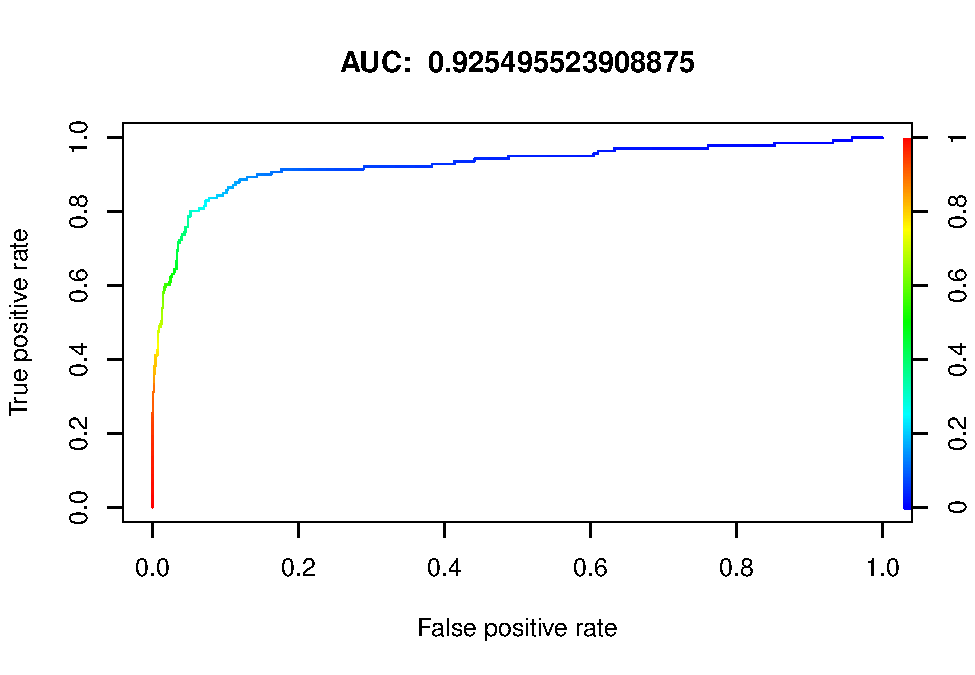
\includegraphics{R_FinalReport_files/figure-latex/unnamed-chunk-44-1.pdf}

\hypertarget{ux5229ux7528caretux5305ux6bd4ux8f83rocux66f2ux7ebf}{%
\subsubsection{利用caret包比较ROC曲线}\label{ux5229ux7528caretux5305ux6bd4ux8f83rocux66f2ux7ebf}}

\begin{Shaded}
\begin{Highlighting}[]
\CommentTok{#install.packages("pROC")}

\KeywordTok{library}\NormalTok{(}\StringTok{"pROC"}\NormalTok{)}
\end{Highlighting}
\end{Shaded}

\begin{verbatim}
## Type 'citation("pROC")' for a citation.
\end{verbatim}

\begin{verbatim}
## 
## Attaching package: 'pROC'
\end{verbatim}

\begin{verbatim}
## The following objects are masked from 'package:stats':
## 
##     cov, smooth, var
\end{verbatim}

\begin{Shaded}
\begin{Highlighting}[]
\CommentTok{#训练控制方法}
\NormalTok{control=}\KeywordTok{trainControl}\NormalTok{(}\DataTypeTok{method=}\StringTok{"repeatedcv"}\NormalTok{,}
                     \DataTypeTok{number=}\DecValTok{10}\NormalTok{,}
                     \DataTypeTok{repeats=}\DecValTok{3}\NormalTok{,}
                     \DataTypeTok{classProbs=}\OtherTok{TRUE}\NormalTok{,}
                     \DataTypeTok{summaryFunction =}\NormalTok{ twoClassSummary)}

\CommentTok{#使用glm在训练数据集上训练一个分类器}
\NormalTok{glm.model=}\StringTok{ }\KeywordTok{train}\NormalTok{(churn}\OperatorTok{~}\NormalTok{.,}
                 \DataTypeTok{data=}\NormalTok{trainset,}
                 \DataTypeTok{method=}\StringTok{"glm"}\NormalTok{,}
                 \DataTypeTok{metric=}\StringTok{"ROC"}\NormalTok{,}
                 \DataTypeTok{trControl=}\NormalTok{control)}

\CommentTok{#使用svm在训练数据集上训练一个分类器}
\NormalTok{svm.model=}\KeywordTok{train}\NormalTok{(churn }\OperatorTok{~}\StringTok{ }\NormalTok{.,}
                \DataTypeTok{data =}\NormalTok{ trainset,}
                \DataTypeTok{method=}\StringTok{"svmRadial"}\NormalTok{,}
                \DataTypeTok{metric=}\StringTok{"ROC"}\NormalTok{,}
                \DataTypeTok{trControl =}\NormalTok{ control)}
\end{Highlighting}
\end{Shaded}

\begin{enumerate}
\def\labelenumi{\arabic{enumi}.}
\setcounter{enumi}{4}
\tightlist
\item
  查看rpart在训练数据上的运行情况
\end{enumerate}

\begin{Shaded}
\begin{Highlighting}[]
\NormalTok{rpart.model =}\StringTok{ }\KeywordTok{train}\NormalTok{(churn }\OperatorTok{~}\StringTok{ }\NormalTok{.,}
                    \DataTypeTok{data =}\NormalTok{ trainset,}
                    \DataTypeTok{method=}\StringTok{"rpart"}\NormalTok{,}
                    \DataTypeTok{metric=}\StringTok{"ROC"}\NormalTok{,}
                    \DataTypeTok{trControl=}\NormalTok{control)}
\end{Highlighting}
\end{Shaded}

\begin{enumerate}
\def\labelenumi{\arabic{enumi}.}
\setcounter{enumi}{5}
\tightlist
\item
  使用不同的已训练好的模型分别进行预测
\end{enumerate}

\begin{Shaded}
\begin{Highlighting}[]
\NormalTok{glm.probs  =}\KeywordTok{predict}\NormalTok{(glm.model,}
\NormalTok{                  testset[, }\OperatorTok{!}\StringTok{ }\KeywordTok{names}\NormalTok{(testset) }\OperatorTok\StringTok{ }\KeywordTok{c}\NormalTok{(}\StringTok{"churn"}\NormalTok{)],}
                  \DataTypeTok{type=} \StringTok{"prob"}\NormalTok{)}
\end{Highlighting}
\end{Shaded}

\begin{verbatim}
## Warning in predict.lm(object, newdata, se.fit, scale = 1, type = if (type == :
## prediction from a rank-deficient fit may be misleading
\end{verbatim}

\begin{Shaded}
\begin{Highlighting}[]
\NormalTok{svm.probs  =}\KeywordTok{predict}\NormalTok{(svm.model,}
\NormalTok{                  testset[, }\OperatorTok{!}\StringTok{ }\KeywordTok{names}\NormalTok{(testset) }\OperatorTok\StringTok{ }\KeywordTok{c}\NormalTok{(}\StringTok{"churn"}\NormalTok{)],}
                  \DataTypeTok{type=} \StringTok{"prob"}\NormalTok{)}
\NormalTok{rpart.probs=}\KeywordTok{predict}\NormalTok{(rpart.model,}
\NormalTok{                  testset[, }\OperatorTok{!}\StringTok{ }\KeywordTok{names}\NormalTok{(testset) }\OperatorTok\StringTok{ }\KeywordTok{c}\NormalTok{(}\StringTok{"churn"}\NormalTok{)],}
                  \DataTypeTok{type=} \StringTok{"prob"}\NormalTok{)}
\end{Highlighting}
\end{Shaded}

\begin{enumerate}
\def\labelenumi{\arabic{enumi}.}
\setcounter{enumi}{6}
\tightlist
\item
  生成ROC曲线
\end{enumerate}

\begin{Shaded}
\begin{Highlighting}[]
\NormalTok{glm.ROC=}\KeywordTok{roc}\NormalTok{(}\DataTypeTok{response=}\NormalTok{testset[,}\KeywordTok{c}\NormalTok{(}\StringTok{"churn"}\NormalTok{)],}
            \DataTypeTok{predictor=}\NormalTok{glm.probs}\OperatorTok{$}\NormalTok{yes,}
            \DataTypeTok{levels=}\KeywordTok{levels}\NormalTok{(testset[,}\KeywordTok{c}\NormalTok{(}\StringTok{"churn"}\NormalTok{)]))}
\end{Highlighting}
\end{Shaded}

\begin{verbatim}
## Setting direction: controls > cases
\end{verbatim}

\begin{Shaded}
\begin{Highlighting}[]
\KeywordTok{plot}\NormalTok{(glm.ROC,}\DataTypeTok{type=}\StringTok{"S"}\NormalTok{,}\DataTypeTok{col=}\StringTok{"red"}\NormalTok{)}


\NormalTok{svm.ROC=}\KeywordTok{roc}\NormalTok{(}\DataTypeTok{response=}\NormalTok{testset[,}\KeywordTok{c}\NormalTok{(}\StringTok{"churn"}\NormalTok{)],}
            \DataTypeTok{predictor=}\NormalTok{svm.probs}\OperatorTok{$}\NormalTok{yes,}
            \DataTypeTok{levels=}\KeywordTok{levels}\NormalTok{(testset[,}\KeywordTok{c}\NormalTok{(}\StringTok{"churn"}\NormalTok{)]))}
\end{Highlighting}
\end{Shaded}

\begin{verbatim}
## Setting direction: controls > cases
\end{verbatim}

\begin{Shaded}
\begin{Highlighting}[]
\KeywordTok{plot}\NormalTok{(svm.ROC,}\DataTypeTok{add=}\OtherTok{TRUE}\NormalTok{,}\DataTypeTok{col=}\StringTok{"green"}\NormalTok{)}


\NormalTok{rpart.ROC=}\KeywordTok{roc}\NormalTok{(}\DataTypeTok{response=}\NormalTok{testset[,}\KeywordTok{c}\NormalTok{(}\StringTok{"churn"}\NormalTok{)],}
            \DataTypeTok{predictor=}\NormalTok{rpart.probs}\OperatorTok{$}\NormalTok{yes,}
            \DataTypeTok{levels=}\KeywordTok{levels}\NormalTok{(testset[,}\KeywordTok{c}\NormalTok{(}\StringTok{"churn"}\NormalTok{)]))}
\end{Highlighting}
\end{Shaded}

\begin{verbatim}
## Setting direction: controls > cases
\end{verbatim}

\begin{Shaded}
\begin{Highlighting}[]
\KeywordTok{plot}\NormalTok{(rpart.ROC,}\DataTypeTok{add=}\OtherTok{TRUE}\NormalTok{,}\DataTypeTok{col=}\StringTok{"blue"}\NormalTok{)}
\end{Highlighting}
\end{Shaded}

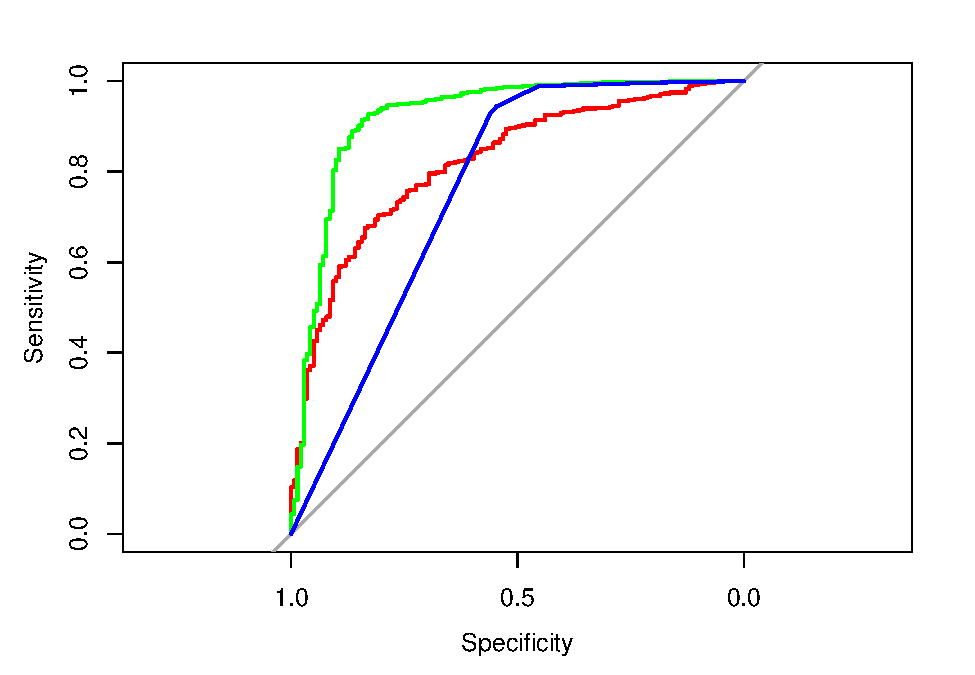
\includegraphics{R_FinalReport_files/figure-latex/unnamed-chunk-48-1.pdf}

\hypertarget{ux5229ux7528caretux5305ux6bd4ux8f83ux6a21ux578bux6027ux80fdux5deeux5f02}{%
\subsubsection{利用caret包比较模型性能差异}\label{ux5229ux7528caretux5305ux6bd4ux8f83ux6a21ux578bux6027ux80fdux5deeux5f02}}

重采样的得到每一个匹配模型的统计信息,包括ROC、灵敏度、特异度。

\begin{enumerate}
\def\labelenumi{\arabic{enumi}.}
\tightlist
\item
  重采样
\end{enumerate}

\begin{Shaded}
\begin{Highlighting}[]
\NormalTok{cv.values=}\KeywordTok{resamples}\NormalTok{(}\KeywordTok{list}\NormalTok{(}\DataTypeTok{glm=}\NormalTok{glm.model,}
                         \DataTypeTok{svm=}\NormalTok{svm.model,}
                         \DataTypeTok{rpart=}\NormalTok{rpart.model))}
\KeywordTok{summary}\NormalTok{(cv.values)}
\end{Highlighting}
\end{Shaded}

\begin{verbatim}
## 
## Call:
## summary.resamples(object = cv.values)
## 
## Models: glm, svm, rpart 
## Number of resamples: 30 
## 
## ROC 
##            Min.   1st Qu.    Median      Mean   3rd Qu.      Max. NA's
## glm   0.7393764 0.7914810 0.8097574 0.8114992 0.8321514 0.9034040    0
## svm   0.8287549 0.8785213 0.8924306 0.8916343 0.9108113 0.9384891    0
## rpart 0.5715885 0.6851976 0.7424457 0.7415887 0.8042699 0.8567483    0
## 
## Sens 
##             Min.   1st Qu.    Median      Mean   3rd Qu.      Max. NA's
## glm   0.08823529 0.1764706 0.2058824 0.2203641 0.2573529 0.4117647    0
## svm   0.48571429 0.5294118 0.6029412 0.5916807 0.6258403 0.7352941    0
## rpart 0.14705882 0.3235294 0.4201681 0.4297199 0.5514706 0.6857143    0
## 
## Spec 
##            Min.   1st Qu.    Median      Mean   3rd Qu.      Max. NA's
## glm   0.9543147 0.9644670 0.9695431 0.9709335 0.9796954 0.9898990    0
## svm   0.9492386 0.9695431 0.9772215 0.9761686 0.9847716 1.0000000    0
## rpart 0.9492386 0.9709275 0.9796954 0.9777009 0.9848485 0.9949239    0
\end{verbatim}

\begin{enumerate}
\def\labelenumi{\arabic{enumi}.}
\setcounter{enumi}{2}
\tightlist
\item
  重采样在ROC曲线度量中的结果
\end{enumerate}

\begin{Shaded}
\begin{Highlighting}[]
\KeywordTok{dotplot}\NormalTok{(cv.values,}\DataTypeTok{metrics=}\StringTok{"ROC"}\NormalTok{)}
\end{Highlighting}
\end{Shaded}

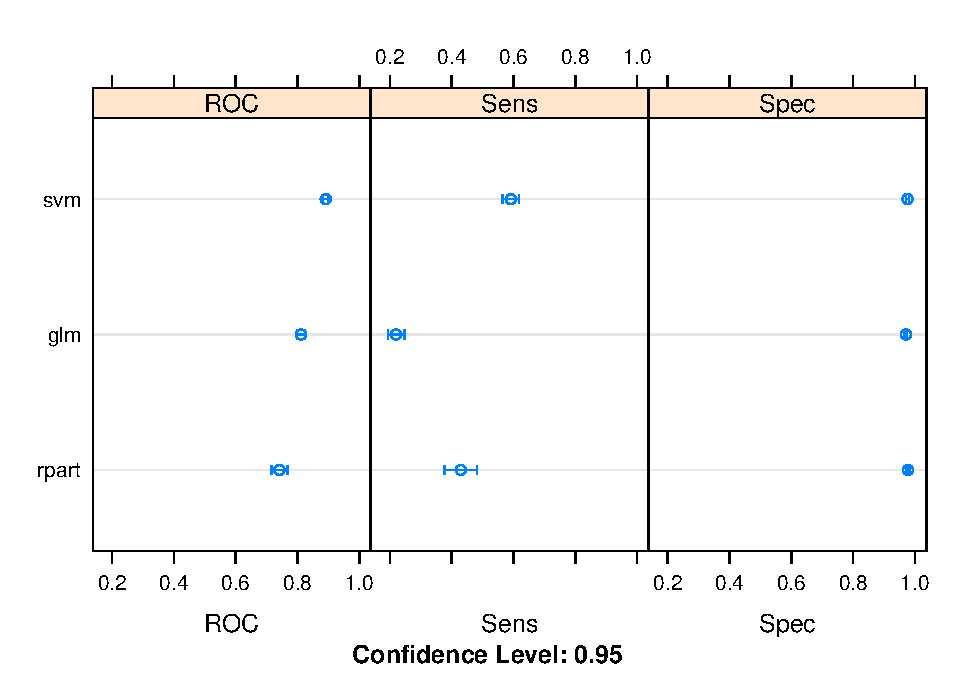
\includegraphics{R_FinalReport_files/figure-latex/unnamed-chunk-50-1.pdf}

\begin{enumerate}
\def\labelenumi{\arabic{enumi}.}
\setcounter{enumi}{3}
\tightlist
\item
  箱线绘制重采样结果
\end{enumerate}

\begin{Shaded}
\begin{Highlighting}[]
\KeywordTok{bwplot}\NormalTok{(cv.values,}\DataTypeTok{layout=}\KeywordTok{c}\NormalTok{(}\DecValTok{3}\NormalTok{,}\DecValTok{1}\NormalTok{))}
\end{Highlighting}
\end{Shaded}

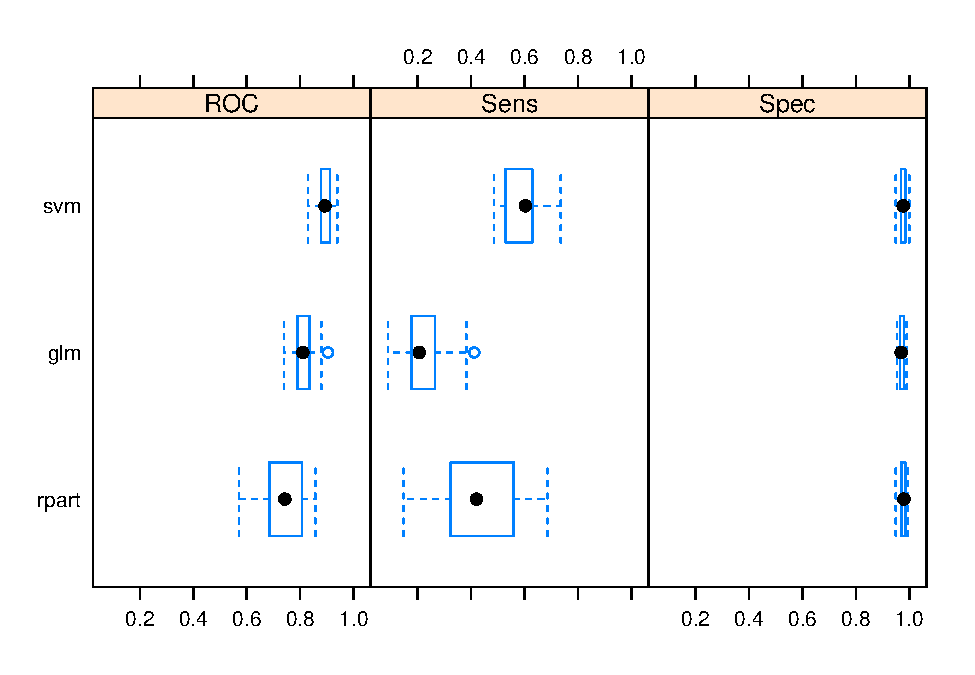
\includegraphics{R_FinalReport_files/figure-latex/unnamed-chunk-51-1.pdf}

\hypertarget{ux53c2ux8003ux6587ux732e}{%
\section{参考文献}\label{ux53c2ux8003ux6587ux732e}}

{[}1{]}CHIU Y-W. Machine Learning with R Cookbook{[}M{]}. Packt
Publishing Ltd, 2015.

\hypertarget{ux9644ux5f55ux4ee3ux7801}{%
\section{附录(代码)}\label{ux9644ux5f55ux4ee3ux7801}}

(将以文件形式附在压缩包内)

\end{document}
